%==============================================================================
% Sjabloon poster bachproef
%==============================================================================
% Gebaseerd op document class `a0poster' door Gerlinde Kettl en Matthias Weiser
% Aangepast voor gebruik aan HOGENT door Jens Buysse en Bert Van Vreckem

\documentclass[a0,portrait]{hogent-poster}

\usepackage{enumitem}

% Info over de opleiding
\course{Bachelorproef}
\studyprogramme{TOEGEPASTE INFORMATICA}
\academicyear{2024-2025}
\institution{Hogeschool Gent, Valentin Vaerwyckweg 1, 9000 Gent}

% Info over de bachelorproef
\title{Integratie en vervanging van het DECT-\-systeem met 5G-\-technologie voor zorg-\-simulaties binnen HOGENT}
\author{Maarten Adriaenssens}
\email{maarten.adriaenssens@student.hogent.be}
\supervisor{Lena De Mol}
\cosupervisor{Thomas Cuelenaere (HOGENT), Jens Buysse (CityMesh) en Max Dekoninck (CityMesh)}

% Indien ingevuld, wordt deze informatie toegevoegd aan het einde van de
% abstract. Zet in commentaar als je dit niet wilt.
\specialisation{Systeem- en Netwerkbeheer}
\keywords{Gezondheidszorg, 5G, DECT-systeem, privaat netwerk}
% \projectrepo{https://github.com/Maarten-Adriaenssens/latex-hogent-bachproef}

\begin{document}

\maketitle

\begin{abstract}


% It's only a model.
% You don't vote for kings. Who's that then? We found them. Ni! Ni! Ni! Ni!
% The nose? On second thoughts, let's not go there. It is a silly place. Bloody Peasant! And the hat. She's a witch! Where'd you get the coconuts?

Deze bachelorpref onderzoekt de mogelijke communicatietechnologieën die kunnen worden ingezet om het huidige DECT-systeem te vervangen. Het doel is om een kwaliteitsvol alternatief te bieden voor de vervanging van het DECT-systeem. Zo wordt er een oplijsting gemaakt van de vereisten en deze afgetoetst met nieuwe technologieën. De technologieën die worden bekeken zijn onder andere: DECT, ULE, VoIP en 5G. Verder bevat het onderzoek in deze bachelorproef ook een Proof of Concept (PoC) van een 5G netwerk-simulatie. Deze PoC wordt ook geautomatiseerd en er wordt gekeken naar de mogelijke stappen om deze simulatie om te zetten naar een praktische realisatie. Uit het onderzoek kan men besluiten dat 5G de beste keuze is op vlak van technologische vervanger van het DECT-systeem. Deze bachelorproef stelt 2 alternatieve opties voor, indien men vandaag een vervanging moet doen met een beperkt budget. De eerste is de nieuwste versie van het DECT-systeem, ook wel het ULE-systeem genoemd. De tweede is een overschakeling naar een combinatie van Wi-Fi en VoIP. Maar in het einde blijft het een afweging tussen de kost en de productiviteitsboost door onder andere de alarmmoeheid vermindering.


\end{abstract}

\begin{multicols}{2} % This is how many columns your poster will be broken into, a portrait poster is generally split into 2 columns

\section{Situering}

Als centrale onderzoeksvraag is er gekozen voor: "Hoe kan de informatie-uitwisseling tussen artsen en verplegend personeel in ziekenhuizen verbeterd worden door het inzetten van nieuwe technologieën ?" \\
Deze wordt beantwoord doorheen de bachelorproef aan de hand van volgende bijvragen:
\begin{itemize}[noitemsep, topsep=0pt, itemsep=1mm, parsep=0pt]
  \item Wat zijn de kenmerken van het DECT-systeem?
  \item Wat is het huidige systeem (met randapparatuur) en wat zijn de nadelen hiervan?
  \item Hoe kan een zorgsituatie worden gesimuleerd?
  \item Welke pogingen zijn al ondernomen om het DECT-systeem als standaard aan te passen?
  \item Wat zijn de minimumvereisten voor technologieën, om als alternatief te kunnen worden beschouwd?
  \item Welke andere communicatiemogelijkheden zijn er die voldoen aan de minimumvereisten?
  \item Welke mogelijke data integratie mogelijkheden hebben de alternatieven?
  \item Vanaf wanneer is het haalbaar om te implementeren op economisch vlak?
\end{itemize}
Het doel van deze bachelorproef is om een antwoord te formuleren op de onderzoeksvraag en een jump-off point te zijn voor verder onderzoek.

\section{Proof of Concept}
Voor het onderzoek, is er een Proof of Concept opgezet. Deze bestaat uit 2 Virtual Machines met hun corresponderende functies zoals hieronder op de figuur geïllustreerd.


\begin{center}
  \captionsetup{type=figure}
  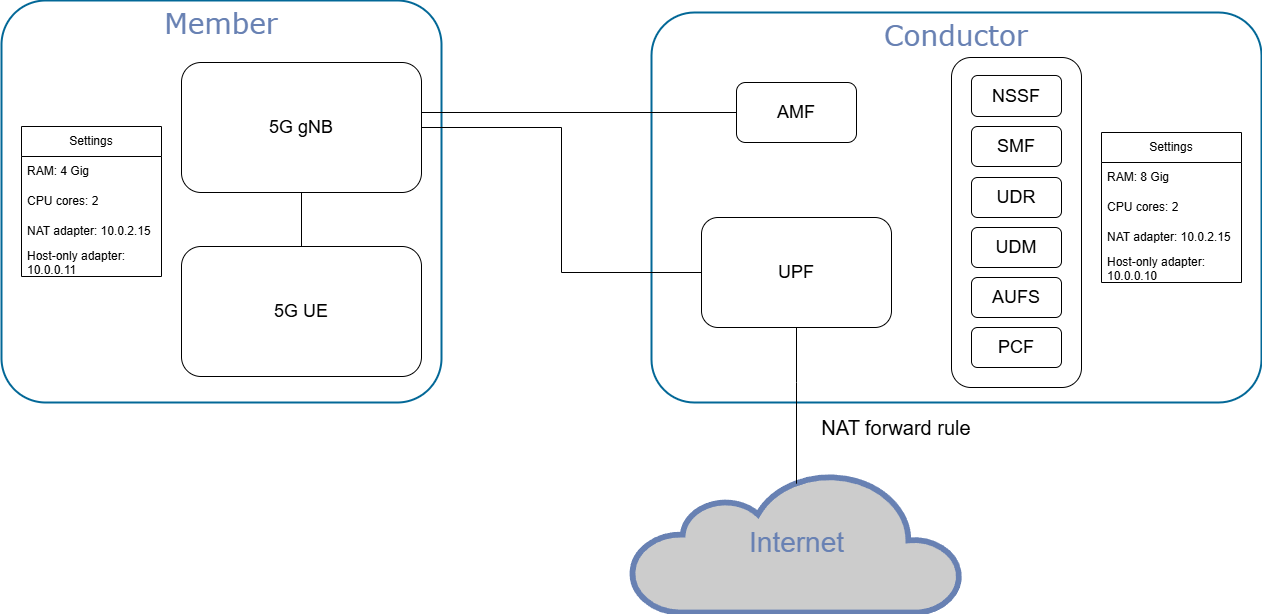
\includegraphics[width=1.0\linewidth]{./graphics/POC-setup.png}
  \captionof{figure}{Proof of Concept Setup (Illustratie)}
\end{center}

Dit netwerk wordt op 2 manieren opgesteld. De eerste is een volledig manuele installatie en configuratie. De tweede is een zo goed al volledig geautomatiseerde opstelling. 
Eenmaal het netwerk tot stand is gekomen wordt dit onderworpen aan verschillende testen. Tijdens deze testen wordt er ook een netwerkopname gemaakt. Dit is hieronder terug te vinden in de screenshot.

\begin{center}
  \captionsetup{type=figure}
  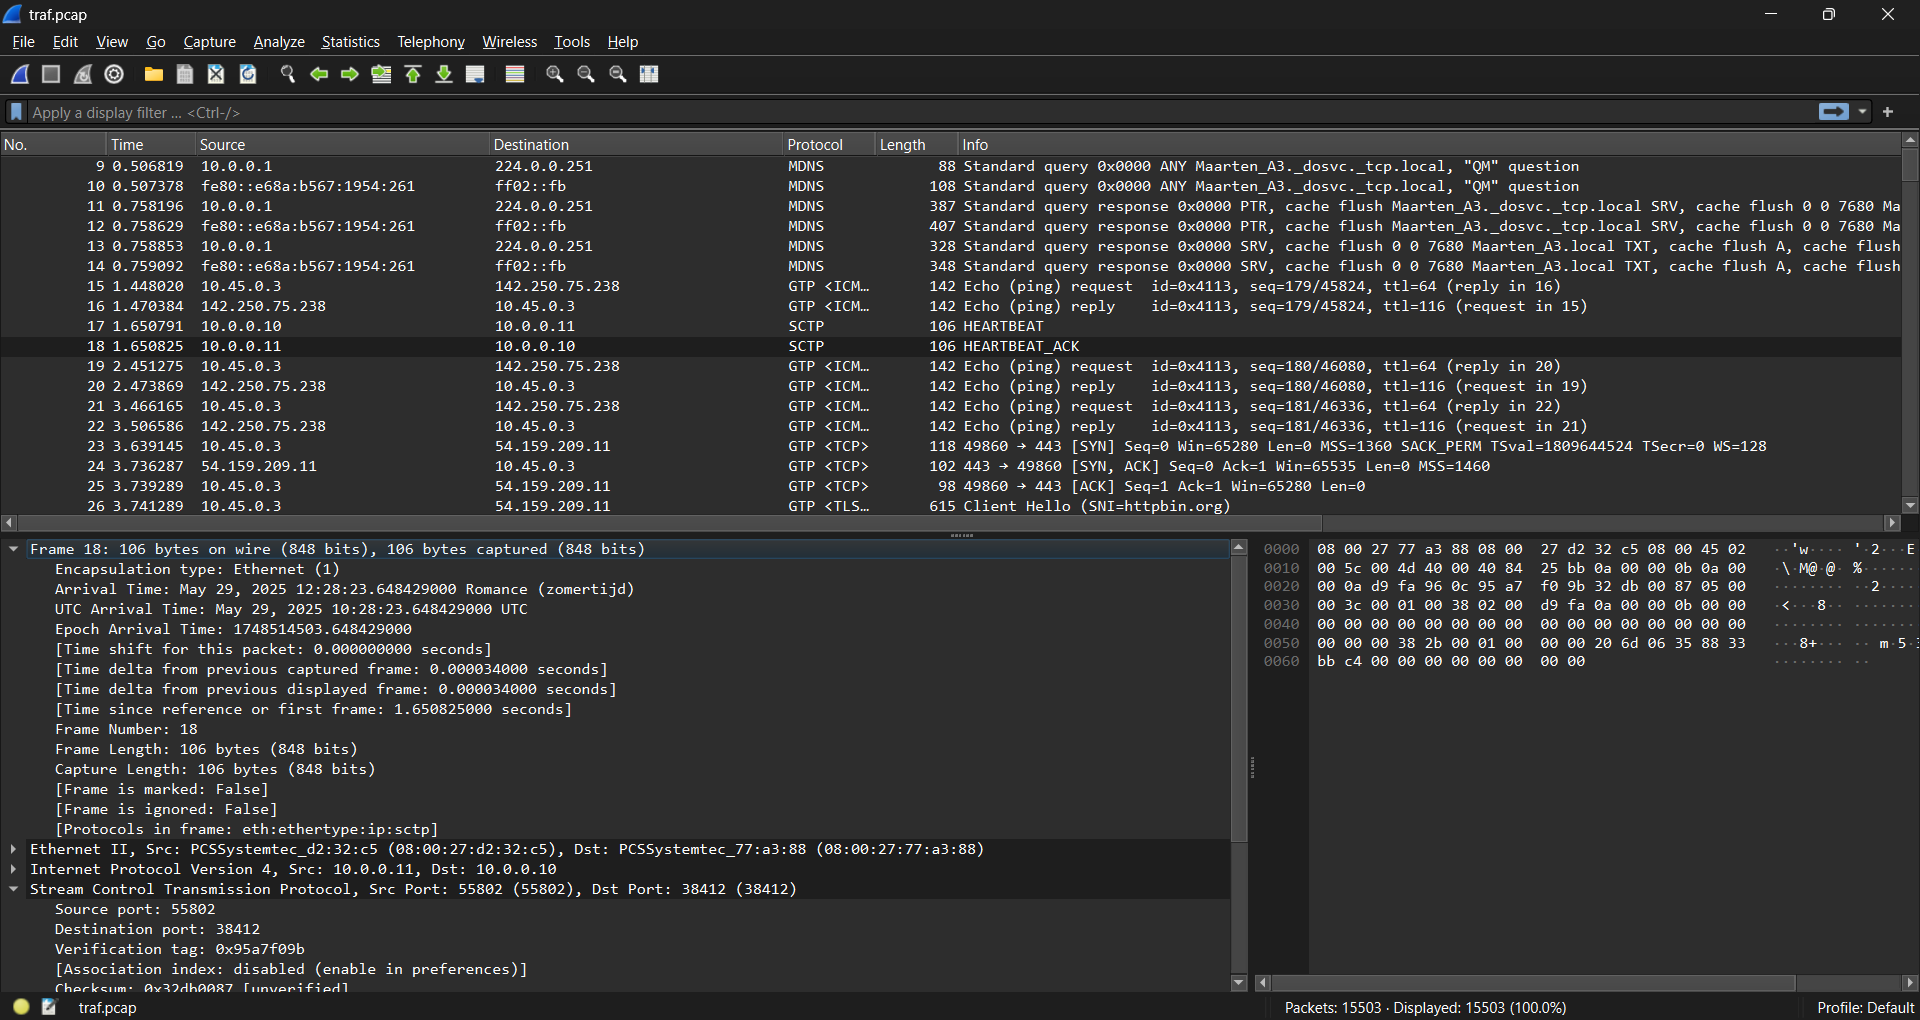
\includegraphics[width=1.0\linewidth]{./graphics/POC-wireshark.png}
  \captionof{figure}{Network capture PoC (Screenshot)}
\end{center}


\section{Resultaten}

In de resultaten wordt er rekening gehouden met alle eigenschappen en beperkingen van de vermeldde technologieën. Hieronder is ook een staafdiagram mee opgenomen om de langdurige kost van een 5G netwerk te kaderen. 
\begin{center}
  \captionsetup{type=figure}
  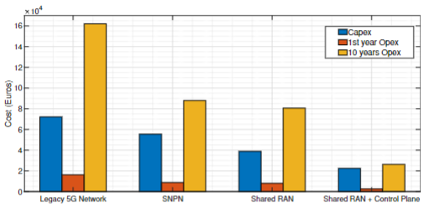
\includegraphics[width=1.0\linewidth]{./graphics/capex-opex.png}
  \captionof{figure}{Vergelijking van CAPEX met OPEX op 1 jaar en op 10 jaar tijd voor 5G netwerken (Door Hilary, 2024) Copyright
2024 van Hilary (2024)}
\end{center}

\section{Conclusies}

De conclusie die wordt getrokken uit het onderzoek is dat een privaat 5G netwerkt theoretisch gezien de beste oplossing is en het nauwste aansluit bij de vereisten. Echter in de realiteit zijn er verschillende extra facetten die zo een keuzes beïnvloeden. Zo is het financieel kader. Een 5G netwerk is een grote investering en kan soms niet worden gedragen. Daarvoor worden er ook alternatieven aangeboden zoals ULE en VoIP.

\section{Toekomstig onderzoek}

Deze bachelorproef dient als springplank voor verder onderzoek en ontwikkeling met als doel het DECT-systeem te vervangen met een kwalitatieve en innovatieve technologie . De eigenschappen van deze technologie hebben als hoofddoel het personeel te ondersteunen en zo de stressfactoren en alarmmoeheid te verminderen of zelfs volledig weg te nemen.
Om dit te testen kan er in de toekomst zeker nog worden samengewerkt met CityMesh en HOGENT. 
\end{multicols}
\end{document}